\clearpage

\section{Детальный обзор LLVM}

LLVM (первоначально аббревиатура расшифровывалась как Low Level Virtual Machine) начался как
исследовательский проект Университета штата Иллинойс. Целью проекта было разработать промежуточное
представление (intermediate representation, IR), основанное на SSA (single static assignment) 
форме, способное описывать конструкции высокоуровневых языков программирования, а так же
универсальный набор оптимизаций над этим представлением. Неполный список проектов, входящих
в состав LLVM, включает в себя:

\begin{enumerate}
\item Ядро библиотеки, содержащее инструменты для работы с LLVM IR, а так же набор
оптимизаций и трансформаций над ним.
\item Clang -- фронтенд для C, C++ и Objective-C.
\item LLDB -- отладчик для C, C++ и Objective-C программ.
\item libc++ -- имплементация стандартной библиотеки C++.
\item OpenMP -- библиотеки времени исполнения для поддержки стандарта OpenMP.
\item LLD -- линковщик.
\item MLIR -- Multi-Level Intermediate Representation, набор библиотек для
создания собственных высокоуровневых промежуточных представлений и трансформаций
над ними. 
\end{enumerate}

\subsection{SSA форма}
Static single assignment form (SSA) -- промежуточное представление, в котором
значения переменным присваиваются лишь один раз. Используется компиляторами для
упрощения процесса оптимизации программного кода. Изменяемость переменных может
достигаться двумя путями. Первый -- выделять динамическую память и обновлять
значения операциями чтения и записи в память (\textit{load and store}). Этот
метод использует clang. Однако в таком виде затрудняется статический анализ
памяти (dataflow analysis). Более удобным способом будет добавление суффикса к
имени переменной. В некоторых случаях первая форма может быть приведена ко 
второй с помощью процедуры под названием \textit{memory to register}.
% https://ru.wikipedia.org/wiki/SSA

\subsection{Just-in-Time компиляция}
Компиляция <<на лету>> (англ. \textit{Just-in-time compilation, JIT}) --
один из видов компиляции, когда промежуточное представление программы, 
называемое байт-код, преобразуется в машинные инструкции прямо во время
исполнения программы. В отличие от компиляции перед выполнением (англ. 
\textit{Ahead-of-time compilation, AOT}), JIT позволяет оптимизировать код
программы непосредственно под архитектуру платформы, на которой программа
исполняется, за счет чего достигается повышение производительности. Однако, у
JIT есть недостаток -- увеличенное время запуска программы. В случае, если она
не выполняет сложных вычислений, время запуска и компиляции может превысить 
время работы.
% https://ru.wikipedia.org/wiki/JIT-%D0%BA%D0%BE%D0%BC%D0%BF%D0%B8%D0%BB%D1%8F%D1%86%D0%B8%D1%8F
\subsubsection{ORC JIT}
Одна из реализаций JIT компилятора в LLVM носит название ORC (On Request 
Compiler). ORC предоставляет модульный набор программных интерфейсов для 
построения собственных компиляторов. Среди его возможностей:
\begin{enumerate}
\item \textbf{JIT-компоновка} позволяет линковать релоцируемые объекты во время
исполнения программы.
\item \textbf{Компиляция LLVM IR} непосредственно в машинный код.
\item \textbf{Упереждающая и <<ленивая>> компиляция} (англ. \textit{eager and
lazy compilation}). В первом случае вся программа компилируется непосредственно
перед запуском программы и сохраняется в оперативной памяти. Во втором случае
код каждой процедуры компилируется непосредственно перед её вызовом.
\item \textbf{Многопоточная компиляция}.
\end{enumerate}
% https://llvm.org/docs/ORCv2.html

\subsection{Оптимизации во время компоновки}
% https://ru.wikipedia.org/wiki/%D0%9A%D0%BE%D0%BC%D0%BF%D0%BE%D0%BD%D0%BE%D0%B2%D1%89%D0%B8%D0%BA
\subsubsection{ThinLTO}
% https://clang.llvm.org/docs/ThinLTO.html
% http://blog.llvm.org/2016/06/thinlto-scalable-and-incremental-lto.html

\subsection{Clang}
% https://www.youtube.com/watch?v=5kkMpJpIGYU
% http://llvm.org/devmtg/2019-10/talk-abstracts.html#tut8
\subsubsection{Драйвер}
\subsubsection{Абстрактное синтаксическое дерево}
\subsubsection{Генерация кода}

\subsection{MLIR}
% https://mlir.llvm.org/
% http://llvm.org/devmtg/2019-04/talks.html#Keynote_1
\subsubsection{Диалекты}
% https://www.youtube.com/watch?v=ff3ngdvUang&feature=youtu.be
\begin{figure}[h]
    \centering
    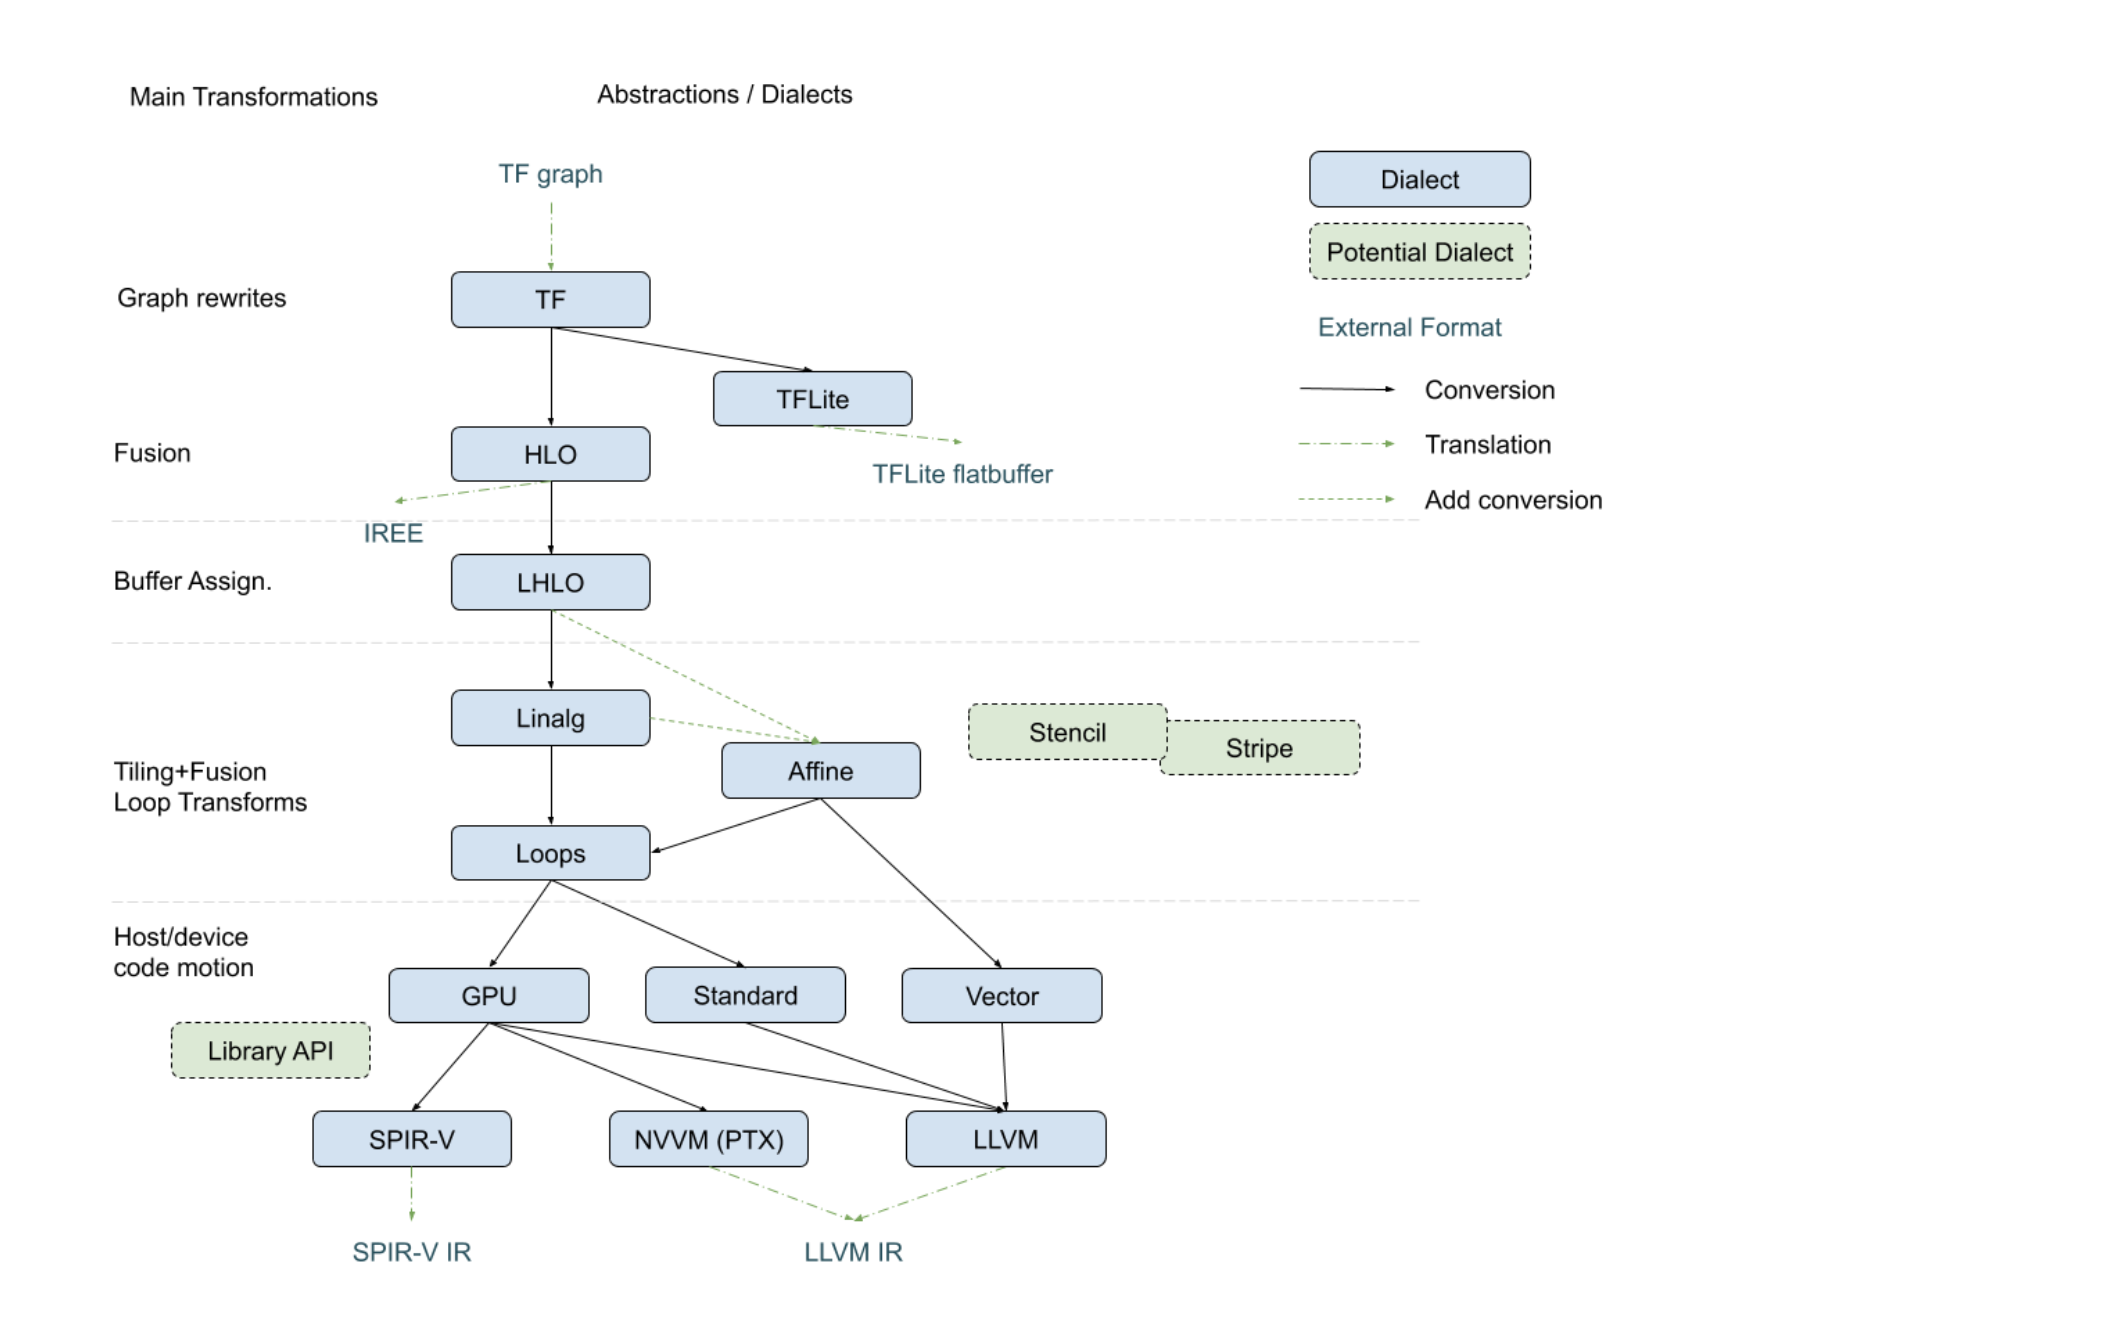
\includegraphics[width=\textwidth]{mlir_vector_dialect.png}
    \caption{Пример взаимодействия диалектов. Источник 
   % https://docs.google.com/presentation/d/1P-j1GrH6Q5gLBjao0afQ-GfvcAeF-QU4GXXeSy0eJ9I/edit#slide=id.p
    }
    \label{fig:mlir_vector_dialect}
\end{figure}
\subsubsection{Упрощенное полиэдральное представление}
% https://mlir.llvm.org/docs/Dialects/Affine/
